\subsection{Key Management Lifecycle}\label{sec:key_management:lifecycle}

The key management lifecycle considers 4 main key states (\Cref{fig:lifecycle}): \textbf{pre-operational} (when keys are not available for use yet), \textbf{operational} (when keys are available for use), \textbf{post-operational} (when keys are available for special purposes only), and \textbf{destroyed} (when keys are no longer available). Each key state is then composed of \textbf{one or more phases}, such as generation, usage, revocation, and destruction of keys. Below, we present each of these phases, describing inherent protocols, algorithms, and best practices.

\remarkBlock{Applicability of key management lifecycle in \Cref{fig:lifecycle}}{Intuitively, not all of the key states and phases described below may be applicable or relevant to all systems. Similarly, different key management lifecycles designed for different systems may consider different key states and phases (e.g.., key suspension) \cite{menezes_handbook_1997}.}

\subsubsection{Pre-Operational Key State}\label{sec:key_management:lifecycle:pre}

\begin{figure}[t!]
	\begin{center}
		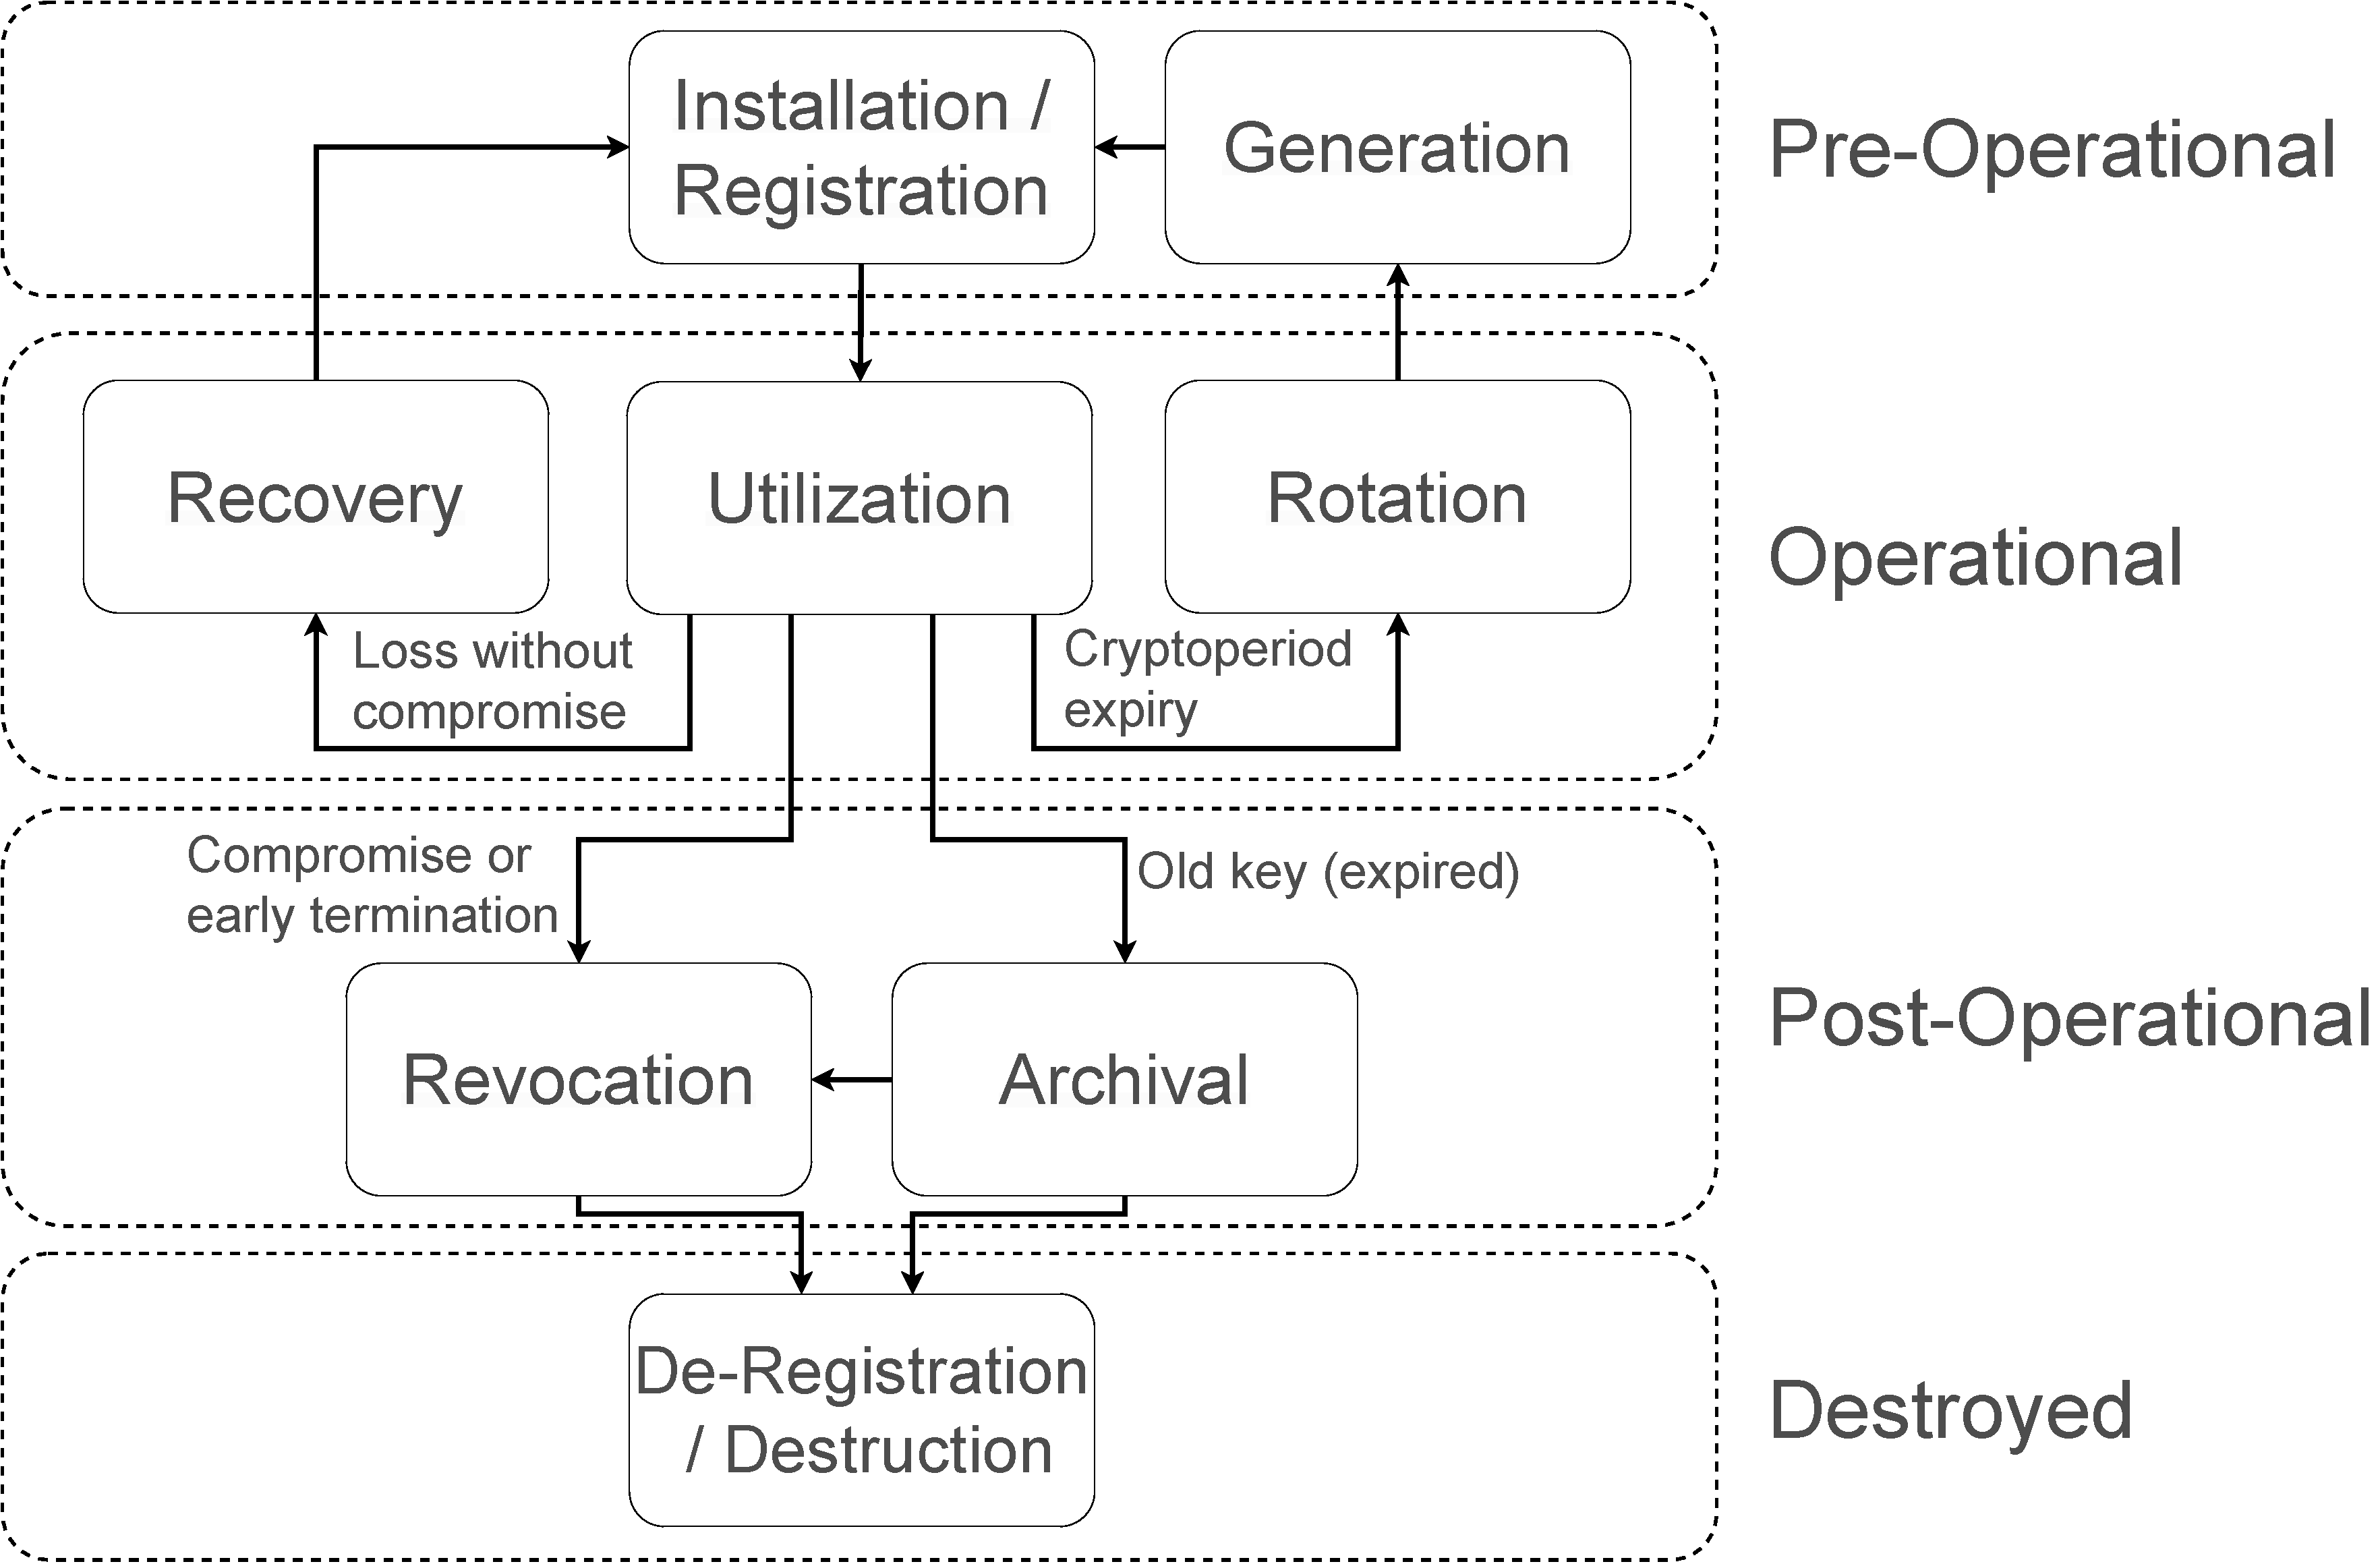
\includegraphics[width=1\linewidth]{resources/pdf/lifecycle.pdf}
		\caption{Key states and phases in the key management lifecycle}
		\label{fig:lifecycle}
	\end{center}
\end{figure}

In this key state, a key has been generated but is not available for use yet. Every newly created key is in the pre-operational key state by default.

\remarkBlock{Entity registration and initialization}{Some key management lifecycles (e.g., \cite{menezes_handbook_1997}) may consider two additional phases in the pre-operational key state, i.e., \textbf{entity registration} and \textbf{entity initialization} --- in this case, ``entity'' is the party to whom the key is associated. During registration, the entity's information is inserted in the system; for physical users, this phase usually correspond to the creation of digital identities \cite{temoshok_digital_2022}, while for organizations this phase is usually a prerequisite for acquiring digital certificates \cite{nist_security_2020} (\Cref{sec:binding_keys_to_parties}). The initialization of entities, instead, corresponds to the installation and configuration of required cryptographic appliances (e.g., software applications, ciphers, and hardware-based cryptographic modules).}

\paragraph*{Key Generation.} The generation of keys --- either done locally for personal use or by a \gls{kga} on behalf of other parties --- marks the beginning of key management. \textbf{Key generation} usually consists of a protocol whereby a key is created or derived by one or more interacting parties using a generic \gls{kdf}. At a high level, a \gls{kdf} is an algorithm taking one or more inputs (where some of the inputs are usually secret) and returning as output a key. Common inputs to \gls{kdf} are the output of \gls{rng}, other keys, and secrets such as passwords --- in the latter case, we talk about \gls{pbkdf} (which we describe below). Either directly or indirectly, each of these inputs includes a (more or less good) entropy source.
%TODO (\Cref{future_sec:randomness}).
\glspl{kdf} often involve the use of (keyed cryptographic) hash functions (\Cref{sec:hash_functions}).

\remarkBlock{On the output of \glspl{kdf}}{Depending on the underlying cipher, the output of a \gls{kdf} may either be immediately usable or need further processing (to, e.g., satisfy specific requirements of the cipher to avoid weak keys --- see \Cref{sec:cryptography_basics:keys}). While symmetric ciphers usually present no such requirements, asymmetric ciphers may require their keys to possess specific properties (e.g., the \gls{rsa} cipher requires the generation of two large primes --- see \Cref{sec:asymmetric_cryptography:ciphers:rsa}).}

Detailed information about the context of the generation of keys (e.g., parameters, intended purpose) should be properly logged --- especially for long-term keys. Protocols for key generation may be categorized as follows (\Cref{figure:key_generation_relationship}):

\begin{figure}[t!]
	\begin{center}
		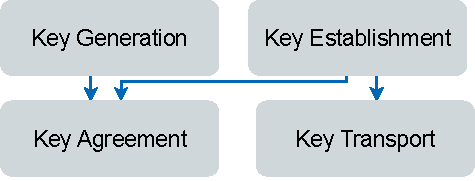
\includegraphics[width=0.5\linewidth]{resources/pdf/key_generation_relationship.pdf}
		\caption{Key generation relationship graph \cite{menezes_handbook_1997}}
		\label{figure:key_generation_relationship}
	\end{center}
\end{figure}

\begin{itemize}
	\item \textbf{key generation}: a protocol whereby a key is created or derived using a generic \gls{kdf}. The most common key generation protocols include:
	\begin{itemize}
		\item the use of dedicated procedures to generate keys for specific algorithms. Such dedicated procedures may be implemented in software or by ad-hoc hardware circuits (\Cref{sec:cryptographic_modules});
		\item the (possibly hierarchical) derivation of a key from another key;
		\item the use of \textbf{mnemonic phrases}, that is, randomly generated sequences of dictionary words that form phrases that can be used as entropy source;
		\exampleBlock{A real-world example of mnemonic phrases usage}{BIP39\footnote{iancoleman/bip39: A web tool for converting BIP39 mnemonic codes (\url{https://github.com/iancoleman/bip39})} --- developed in the context of Bitcoin --- uses mnemonic phrases (also called \textit{seed phrases}) of 12, 18, or 24 words that serves as a human-readable representation of random seeds used to generate private keys.}
		\item the derivation of a (usually symmetric) key from a password or passphrase via a \gls{pbkdf};
	\end{itemize}
	\item \textbf{key establishment}: a protocol whereby a key becomes available to two or more parties;
	\item \textbf{key agreement}: an instance of key generation or key establishment, it is a protocol whereby a key is derived from a function (i.e., a \gls{kdf}) of information contributed by (or associated with) each of the involved parties, such that no party (or subset of parties) alone can predetermine the key while the other parties cannot --- an example of key agreement is \gls{dh} (\Cref{sec:diffie_hellman});
	\item \textbf{key transport}: an instance of key establishment, it is a protocol whereby one party possessing a key --- usually a \gls{kga} --- securely transfers the key to other parties --- an example of key transport are \glspl{kem} (\Cref{sec:key_encapsulation_mechanisms}). Key transport is also called \textbf{key distribution} \cite{barker_recommendation_2020_p1}.
\end{itemize}

\remarkBlock{Mnemonic phrases vs. passwords and passphrases}{Apart from being sequences of characters --- including letters, digits, and possibly other symbols --- mnemonic phrases are a different concept that serves a different purpose with respect to passwords and passphrases. A mnemonic phrase represents a random seed for generating private keys, while a password (or a passphrase) is a word (or sequence of words) kept secret by a user. Passwords are sometimes called \textit{passcodes}, and a password including digits only is usually called \textit{\gls{pin}}. Passphrases are longer than passwords, hence more secure.}

\begin{figure}[t!]
	\begin{center}
		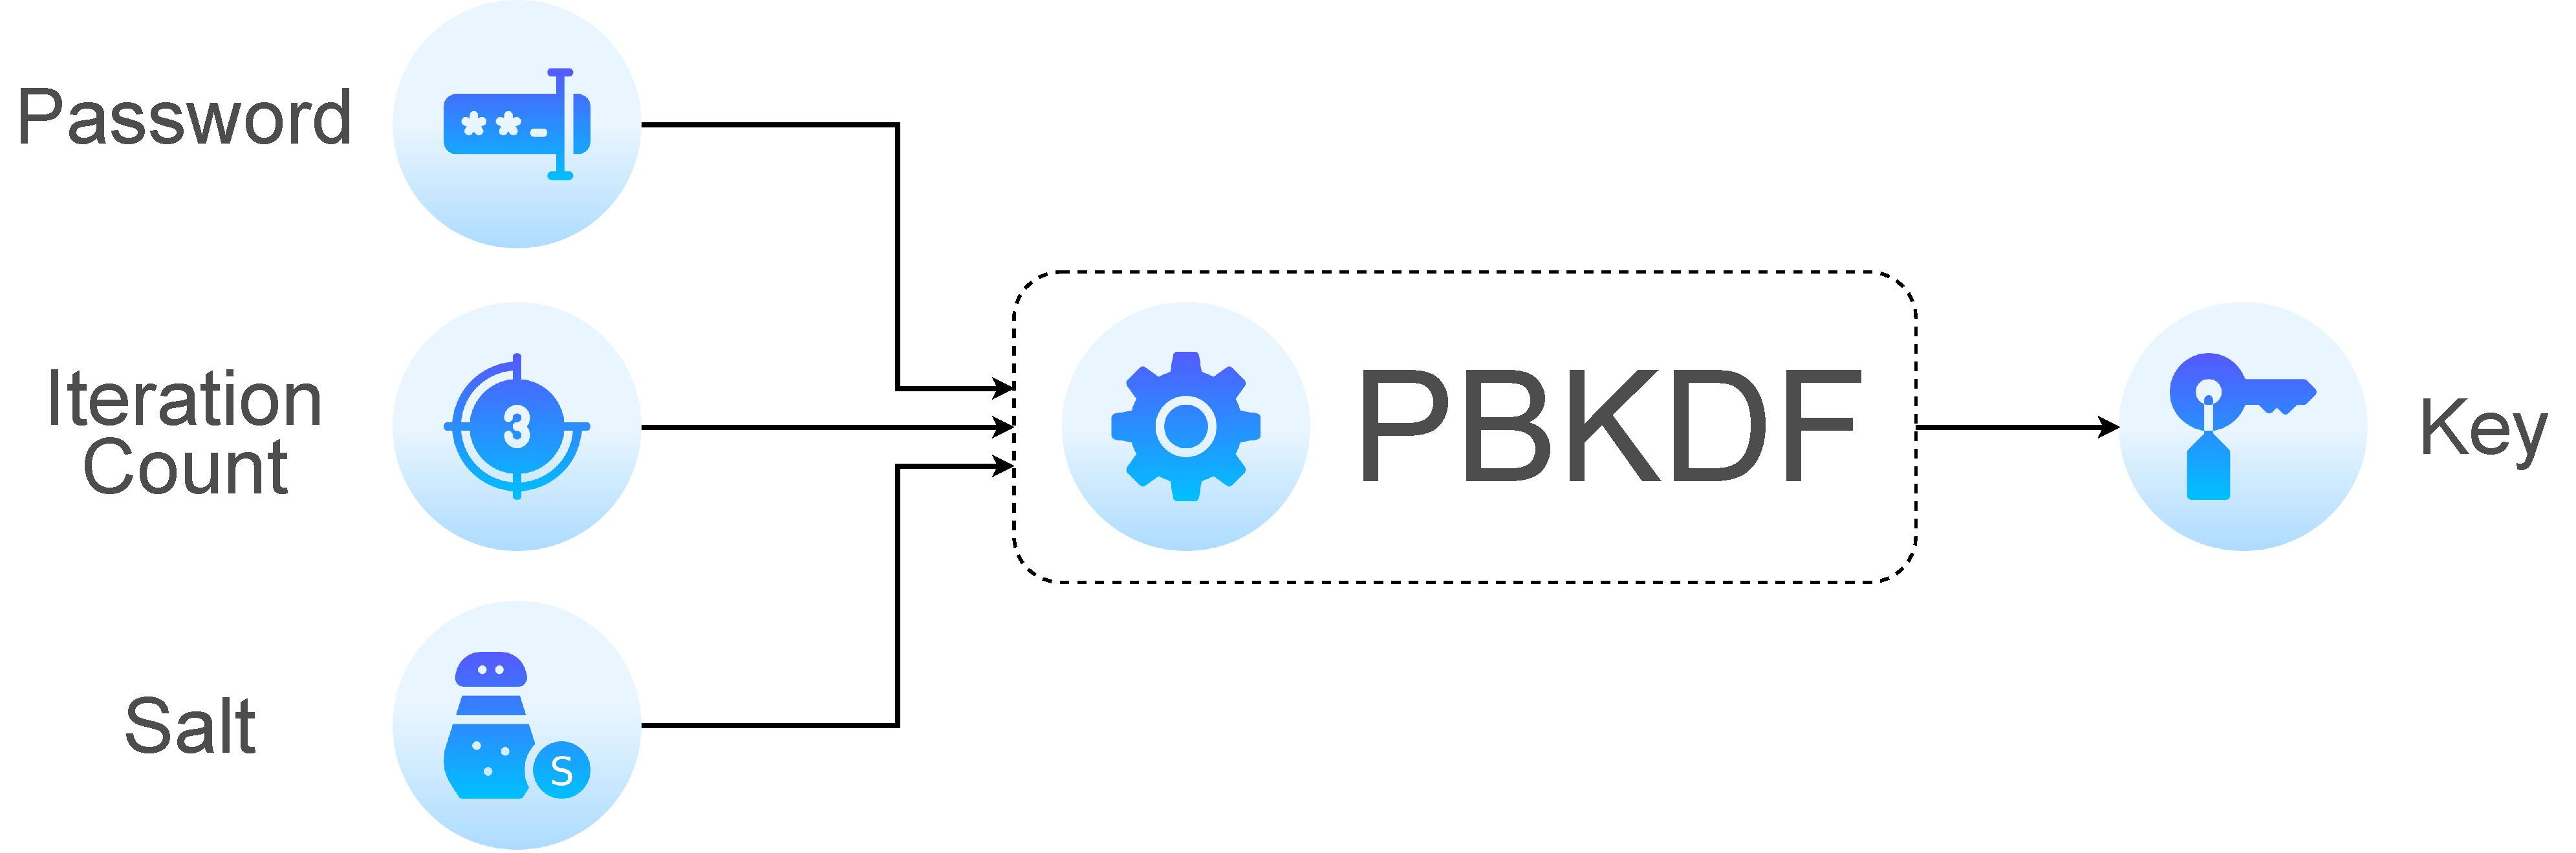
\includegraphics[width=1\linewidth]{resources/pdf/pbkdf.pdf}
		\caption{Generic Password-Based Key Derivation Function}
		\label{fig:pbkdf}
	\end{center}
\end{figure}

\glspl{pbkdf} are a specific instance of \gls{kdf} where one of the inputs is a password (or passphrase). \glspl{pbkdf} are more than simply applying generic \glspl{chf} to the password and use the resulting digest as a key --- otherwise ($i$) they would always return the same key for the same password, ($ii$) attackers may guess (at least trivial) passwords easily using rainbow tables or performing brute force or dictionary attacks \cite{turan_recommendation_2010} (\Cref{sec:cryptographic_security_overview:attacks}), and ($iii$) generic \gls{chf} are efficient, hence they would speed up the aforementioned attacks.

In fact, modern \glspl{pbkdf} usually consider at least 3 inputs (\Cref{fig:pbkdf}): a password, an iteration count, and a salt. The iteration count specifies how many times the (\gls{chf} contained within the) \glspl{pbkdf} is applied --- to make brute force attacks more time-consuming and resource-intensive --- while the salt is a (non-secret and unique) random sequence of bytes that is combined (often concatenated\footnote{More precisely, the salt and the password are not (or at least should not) naively concatenated, as to avoid ambiguities leading to inconsistencies such as \texttt{``password1||1salt'' = ``password11||salt''}. For this reason, salt and password are usually combined in a length-defined or structured way, so that the boundary between password and salt is never ambiguous.}) with the password before being hashed --- to thwart pre-image attacks (\Cref{sec:hash_functions}). Recommended values for iteration count and salt may vary depending on the specific \gls{pbkdf} \cite{turan_recommendation_2010}. 
Finally, besides an iteration count, some \glspl{pbkdf} are also specifically designed to be inefficient or complex to parallelize or execute on GPUs (e.g., Argon2).

\exampleBlock{Real-world examples of \glspl{pbkdf}}{BCRYPT \cite{provos_bcrypt_1999}, Argon2 \cite{biryukov_argon2_2016}, and PBKDF2 \cite{rfc2898} are modern or widely used \gls{pbkdf}.}

\warningBlock{Limitations of \gls{pbkdf}}{One of the main drawbacks of using \glspl{pbkdf} is that passwords tend to have low entropy. It has been estimated that a password of 8 characters including an uppercase and lowercase letter, a symbol, and a digit has 33 bits of entropy, while a random sequence of 8 characters has 52 bits of entropy \cite{kelley_guess_2012}.}

\readBlock{More information on key generation}{The \gls{nist}'s special publication on key generation \cite{barker_recommendation_2020} is an excellent source of more information on key generation.}

\paragraph*{Key Installation and Registration.} After generation, cryptographic material (e.g., keys, digital certificates) needs to be installed onto the devices from which it will be used \textit{entity-side} --- along with suitable metadata; the installation may be either manual (e.g., transfer from disk, read-only device, hardware token) or automated --- granted a secure protocol is executed. Contextually, cryptographic material should also be registered \textit{system-side} (e.g., registering a newly issued digital certificate). Concretely, key registration implies the recording of the related metadata. Whenever possible, the binding of cryptographic material with entities should be cryptographic (e.g., using a \gls{pki}). Note that ephemeral keys and short-lived keys (\Cref{sec:cryptography_basics:keys})) do not need to be registered --- although it is usually recommended to log relevant related information.


\subsubsection{Operational Key State}\label{sec:key_management:lifecycle:operational}

In this key state, a key is available for use for the intended purpose. Keys transition in the operational key state either directly following generation --- if the keys were created for immediate use and the corresponding metadata were correctly associated --- or upon reaching an activation date (e.g., the \texttt{notBefore} date in an X.509 digital certificate for a public-private key pair in a \gls{pki} \cite{rfc5280} --- see \Cref{sec:binding_keys_to_parties:digital_certificate}).


\paragraph*{Key Utilization.} When in the operational key state, a key is available for use and may be either at rest, in transit, or in use; note that a key in use may also simultaneously be in transit and at rest \cite{barker_recommendation_2020_p1}:

\begin{itemize}
	\item \textbf{key at rest}: stored keys should be protected either by specific hardware-based cryptographic modules (\Cref{sec:cryptographic_modules}) or --- when managed by general purpose hardware (e.g., a laptop) --- by software-based keystores, procedural controls, and physical isolation (e.g., secured rooms with isolated equipment). Intuitively, relying on hardware-based cryptographic modules is usually recommended, as it is the usage of key wrapping (\Cref{sec:cryptography_basics:keys}) to preserve the confidentiality and integrity of keys. Furthermore, \glspl{dek} should be stored in a separate location from the associated encrypted data. Finally, the availability of stored keys --- particularly important for long-term keys --- may be guaranteed through backups when possible (the aforementioned recommendations for secure storage of keys apply to their backups as well). A backup always refers to short-term storage during operational use and is usually implemented by duplicating keys;
	\warningBlock{Do not backup long-term private keys for signatures}{As an exception, the backup of private keys used for signatures is generally discouraged by \gls{nist} due to possibly loss of non-repudiation \cite{barker_recommendation_2020_p1}.}
	\item \textbf{key in transit}: a key may be in transit due to a key transport protocol --- hence, the key is being distributed, either manually or automatically, to authorized parties (\Cref{sec:key_management:lifecycle:pre}) --- or due to backup or archival (\Cref{sec:key_management:lifecycle:post}). In any case, key wrapping should be applied to keys in transit --- even if secure communication protocols such as \gls{tls}
	%TODO (\Cref{future_sec:popular_protocols:tls})
	are used;
	\item \textbf{key in use}: the use of keys should occur within (possibly hardware-based) cryptographic modules only and be subject to \gls{ac} policies.
	%TODO (\Cref{future_sec:access_control}).
	Furthermore, it is a best practice to implement monitoring mechanisms to track and log key usage and to regularly review logs to detect unauthorized or suspicious activities.
\end{itemize}

\remarkBlock{On keys splitting}{Keys at rest, in transit, or in use may be split to improve security and reduce risks of compromise using \gls{tss} or \gls{smpc} schemes.
%TODO --- see \Cref{future_sec:secret_sharing_and_threshold_schemes,future_sec:advanced_cryptography:secure_multi_party_computation}, respectively. 
Nonetheless, each share of a key should anyway be protected as just described.}

\begin{figure}[t!]
	\begin{center}
		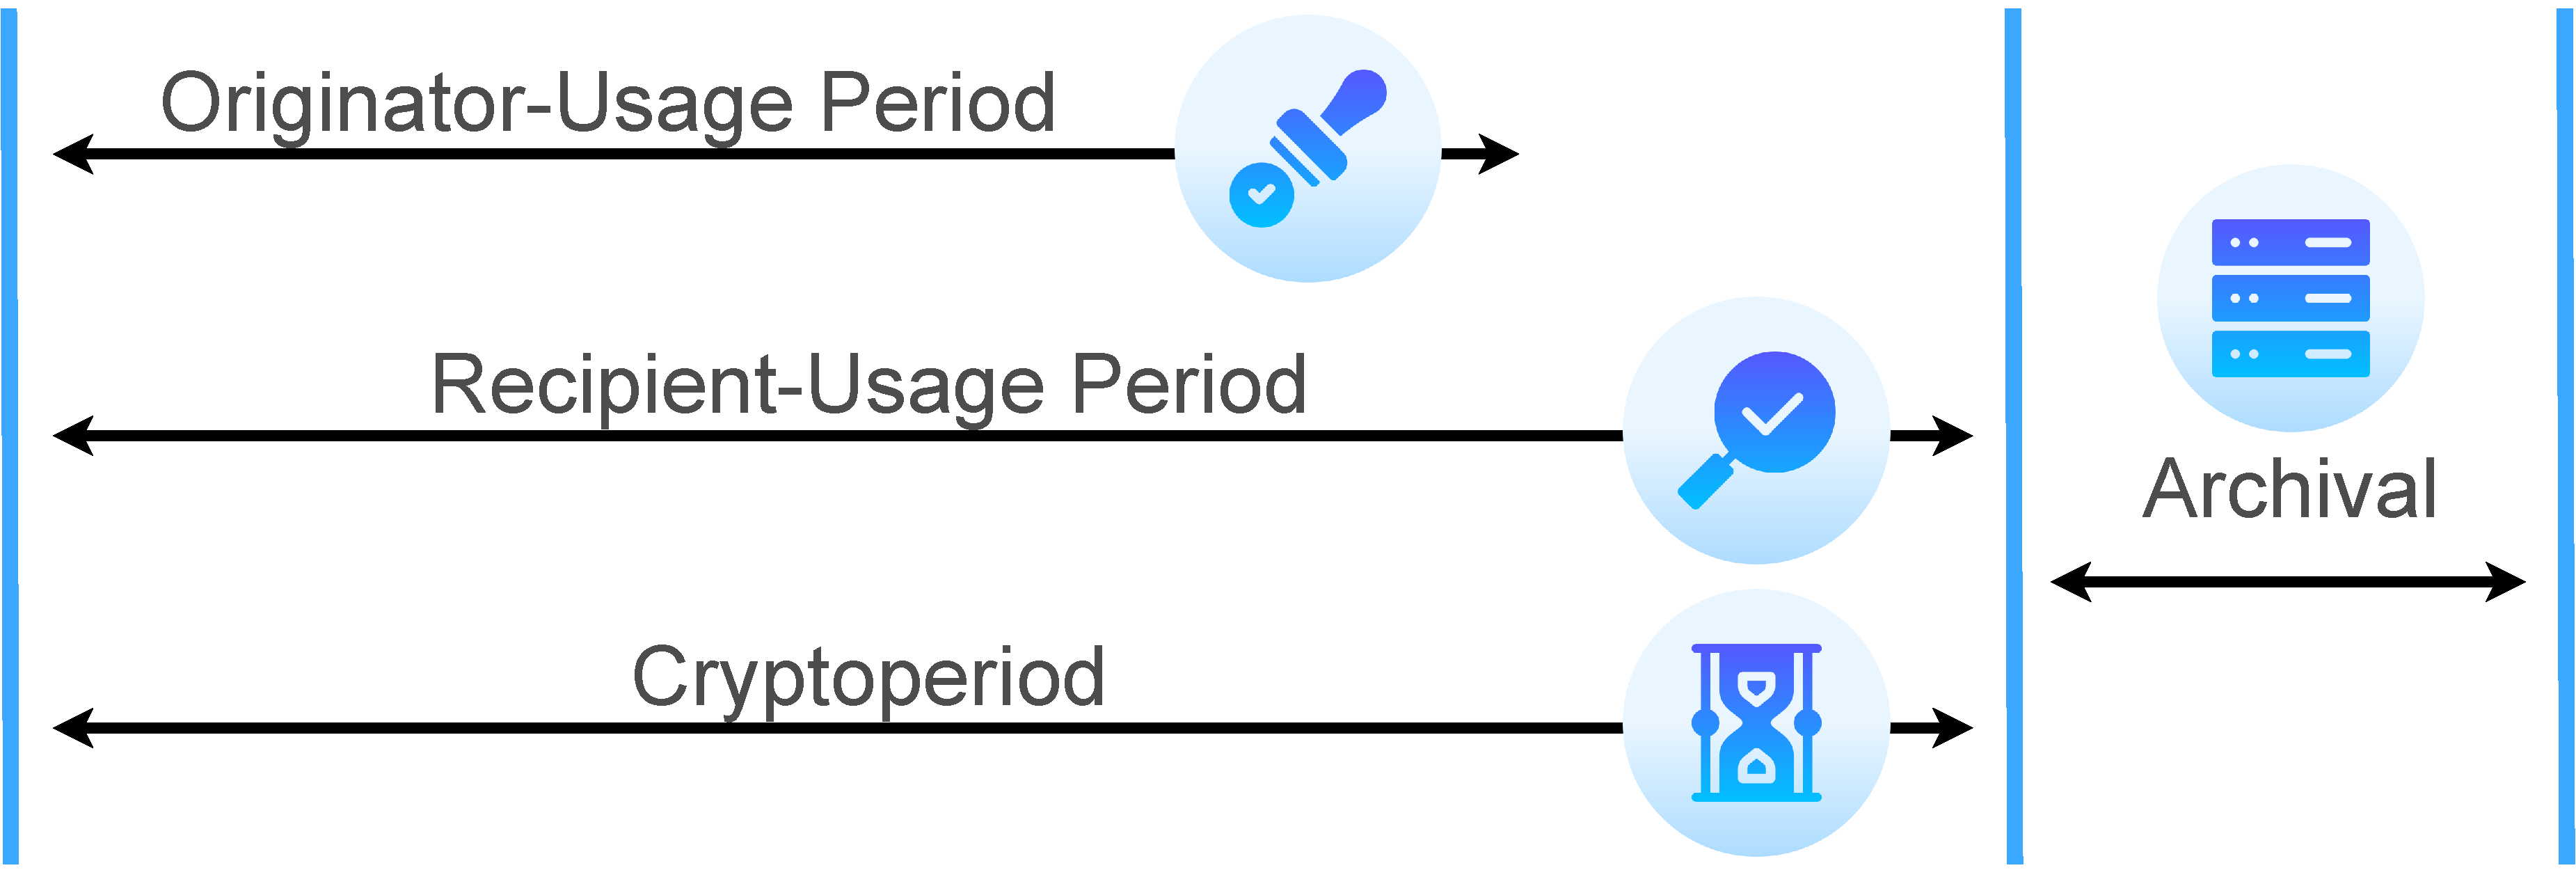
\includegraphics[width=1\linewidth]{resources/pdf/cryptoperiod.pdf}
		\caption{Cryptoperiod and Archival in the Key Management Lifecycle}
		\label{fig:cryptoperiod}
	\end{center}
\end{figure}

All keys have a \textbf{cryptoperiod} --- that is, a time span during which keys are authorized for use --- after which the keys \textit{expire} and should not be used anymore --- except for special purposes. Indeed, over time, keys may be leaked, compromised, or found vulnerable (the keys themselves or their ciphers); defining a cryptoperiod allows for preventing and mitigating these risks and the corresponding security threats. A cryptoperiod may be either temporal (e.g., number of days) or based on the amount of data processed (e.g., encrypted) to limit the amount of information available for cryptanalysis. As shown in \Cref{fig:cryptoperiod}, a cryptoperiod typically comprises an \textbf{originator-usage period} and a \textbf{recipient-usage period}: the former is the period during which keys can apply cryptographic protections (e.g., encryption, creation of digital signatures), while the latter is the period during which keys can process cryptographic protections. The recipient-usage period is usually equivalent to the cryptoperiod, while the originator-usage period is often shorter.

\remarkBlock{How to compute cryptoperiods}{There is no (widely adopted) formula for calculating cryptoperiods exactly, as these depend on several (often subjective) factors such as the sensitivity of the data, the risk of attacks, the cost of generating and distributing new keys (and, possibly, re-encrypting data), the strength of the chosen cipher, the methodology for storing keys, and the size of keys; for more details and some examples, we refer the interested reader to \cite{barker_recommendation_2020_p1}.}

\paragraph*{Key Rotation.} Keys may need to be rotated due to (presumed or real) leakages and the end of their cryptoperiods. When new keys are generated independently of old keys, we talk about \textbf{re-keying}; \textbf{key update} otherwise. Re-keying is often computationally more intensive than key update; for instance, re-keying a \gls{dek} implies re-encrypting the associated data --- either immediately (i.e., \textit{eager re-encryption}) or the first time the data needs to be decrypted (i.e., \textit{lazy re-encryption}). Intuitively, lazy re-encryption does not apply to compromised keys. However, key update entails a higher security risk; for instance, if an attacker compromises a key, knowing the update process, keys derived from the compromised key could easily be determined \cite{barker_recommendation_2020_p1}. In other words, key update is strongly discouraged. In any case, key rotation should be synchronized and happen simultaneously for all instances of the keys being rotated.

\remarkBlock{Key rotation and \gls{pbkdf}}{When a key that has to be rotated was generated through a \glspl{pbkdf}, it is recommended to also change the corresponding password.}

\paragraph*{Key Recovery.} Keys may be lost or become unusable due to, e.g., accidental or intentional modifications and deletions, hardware damage, or corruption. Under the assumption that a lost or unusable key was not compromised, that key may be recovered if deemed necessary either through backups or archives (\Cref{sec:key_management:lifecycle:operational,sec:key_management:lifecycle:post}). Even a compromised key may be recovered, but only for processing (previously existing) cryptographic protections after a careful evaluation of inherent risks. 

\readBlock{More information on key recovery}{Appendix B of the \gls{nist}'s special publication on key management \cite{barker_recommendation_2020_p1} contains further information on key recovery.}

\subsubsection{Post-Operational Key State}\label{sec:key_management:lifecycle:post}

In this key state, a key should be available for use for special purposes only. In particular, keys in this state should not be used for applying cryptographic protections, but only for processing (previously existing) cryptographic protections --- if strictly necessary. For instance, a public key may be used to verify a digital signature created before the cryptoperiod of the corresponding private key ended to settle disputes involving repudiation. Similarly, a \gls{kek} may be used to allow re-encrypting wrapped keys. In general, the use of keys in the post-operational key state should aim at processing cryptographic protections and renewing them with new keys. Keys transition in the post-operational key state when expired (\Cref{sec:key_management:lifecycle:operational}) --- hence, when they need to be archived --- or compromised --- hence, when they need to be revoked. The post-operational key state is sometimes called \textit{deactivated key state} \cite{barker_recommendation_2020_p1}.

\paragraph*{Key Archival.} As shown in \Cref{fig:cryptoperiod}, when (the associated cryptoperiod) expired and not suspected to have been compromised, keys may be archived to be used for the aforementioned special purposes. Archival always refers to long-term storage where post-operational keys --- together with the associated metadata --- are stored offline with the appropriate protections (e.g., key wrapping, \gls{ac} policies). Note that archives may (and should) have backups.

\paragraph*{Key Revocation.} A key may be revoked mainly for 2 reasons: ($i$) the key --- in any key state of phase --- is suspected to have been compromised or ($ii$) the authorized use of the key is terminated before the end of its cryptoperiod (e.g., because the owner of the key has left the system, or the device containing the key has been removed from service) \cite{barker_recommendation_2020_p1}. In both cases, a notification that a key has been revoked should be sent to all entities that have been, are, or would be using the revoked key. The notification should contain at least the identifier of the key, the timestamp, and the motivation for the revocation. The latter is particularly useful to allow recipient entities to determine how to behave toward the revoked key. 

\warningBlock{Revocation of a long-term private key for signatures}{If a public key used for verifying signatures is revoked because its owner left the system, signatures created before the revocation can still be considered trustworthy, hence valid. If the same public key is revoked because of suspected compromise, then there is the need to carefully assess whether to trust previously created signatures; this assessment --- and possible consequent signature verification operations --- should be conducted in a highly controlled environment with a clear image of the possible consequences.} 

A key revoked due to compromise is usually rotated through re-keying (\Cref{sec:key_management:lifecycle:operational}). Finally, the way notifications are broadcasted depends on the key and the underlying system; for instance, \glspl{crl} would be used in the context of a \gls{pki} for asymmetric keys, while a \gls{ckl} may be used for symmetric keys \cite{barker_recommendation_2015}.


\subsubsection{Destroyed Key State}\label{sec:key_management:lifecycle:destroyed}

In this key state, a key is no longer available for use. Keys transition in the destroyed key state --- sometimes also called \textbf{obsolete} --- when created but never used (i.e., directly from the pre-operational phase) or when no longer used for the special purposes considered in the post-operational key state (i.e., for processing previously existing cryptographic protections) or after having being revoked.

\paragraph*{Key De-Registration and Destruction.} When in the destroyed key state, keys need to be de-registered and then destroyed. The de-registration of a key implies marking all related records to indicate that the key was destroyed --- contrary to what one may think, these records should not be deleted, as they may be useful for audit purposes. The destruction of a key implies that all copies of the key --- both in backups and archives --- are destroyed, that is, securely erased so that they cannot be recovered by either physical or electronic means. Key destruction strictly applies to private and secret keys, while public keys may be either retained or destroyed. Finally, a compromise of a destroyed key could be discovered after destruction: in this case, the event should be recorded \cite{barker_profile_2015}.

\remarkBlock{Entity de-registration}{Similarly to key, entities should be de-registered when no longer involved in the system. Records related to a de-registered entity should be properly marked but not deleted.}
